%==============================================================================
\section{Particle Swarm Optimization}
\label{sec:PSO}
%==============================================================================
\textit{Particle Swarm Optimization} (PSO) foi introduzido por Kennedy e Eberhart em 1995~\cite{eberhart1995}, e foi inspirado no comportamento social de organismos biológicos, mais especificamente na habilidade de algumas espécies de animais de trabalhar em conjunto para localizar boas regiões com fontes de alimento, assim como ocorre em cardumes e em bandos de pássaros~\cite{bratton2007}. Em outras palavras, é baseado em um enxame de partículas (\emph{Particle Swarm}) que se movem pelo espaço e se comunicam para determinar uma direção de busca ideal. O PSO tem melhor desempenho computacional para este tipo de problema de otimização de funções não-lineares de alta dimensionalidade com variáveis contínuas, do que outros algoritmos~\cite{eberhart1995,bratton2007,alrashidi2009} e tem menos parâmetros para ajustar, facilitando sua implementação. O PSO vem sendo utilizado com sucesso na solução de problemas da ciência e da engenharia devido à sua simplicidade, eficácia e robustez~\cite{fukuyama1999, ourique2002, sousa2004,van2006,engelbrecht2007, alrashidi2009,rodriguez2014,al2015}. Apresenta como desvantagens, a necessidade de informação do tomador de decisão, parâmetros difíceis de ajustar, e ainda incapacidade de alcançar a Frente de Pareto, principalmente em problemas com multimodalidade, aqueles com múltiplas soluções ótimas, onde algumas podem ser melhores soluções globais e outras melhores soluções locais~\cite{figueiredo2013}, porém adapta-se ao problema abordado.

Cada partícula $ i $ do enxame $ S $ é representada por sua posição e sua velocidade. A posição é um vetor de $ n $ dimensões, cujos componentes representam os parâmetros da função objetivo. As partículas controlam a sua melhor posição $ pbest $ e a melhor posição global $ gbest $, a melhor solução conhecida dentro de sua vizinhança.

Inicialmente, as partículas do enxame possuem posições aleatórias no espaço de busca, obedecendo uma distribuição de probabilidade uniforme. Posteriormente, a posição $ {x_i}\left( t \right) $ de cada partícula $ i $ na iteração $ t $ é modificada por uma velocidade estocástica $ {v_i}\left( t \right) $ que depende da distância que a partícula está da sua melhor solução conhecida e da distância para a melhor solução conhecida dentro de sua vizinhança. Cada partícula $i \in S$ se movimenta em cada dimensão $j \in \left\{ {1,2,..n} \right\}$ do espaço de busca em um instante discreto de tempo $ t $, segundo as Equações~\ref{equa:pso1} e~\ref{equa:pso2}:
\begin{equation}
{\overrightarrow x _i}\left( {t + 1} \right) = {\overrightarrow x _{_i}}\left( t \right) + {\overrightarrow v _i}\left( t \right)
\label{equa:pso1}
\end{equation}
%
\begin{equation}
{\overrightarrow v _i}\left( {t + 1} \right) = w{\overrightarrow v _i}\left( t \right) + {c_1}{r_1}\left( {\overrightarrow x _i^*\left( t \right) - {{\overrightarrow x }_{_i}}\left( t \right)} \right) + {c_2}{r_2}\left( {{{\overrightarrow x }^*}\left( t \right) - {{\overrightarrow x }_{_i}}\left( t \right)} \right)
\label{equa:pso2}
\end{equation}
onde:
$ w $ = inércia

$ c _i $ = coeficiente de aceleração, $i=\left( 1,2 \right)$

$ r _i $ = número aleatório pertencente a uma distribuição de probabilidade uniforme , $i=\left( 1,2 \right)$ e ${r_i} \in \left[ {0,1} \right]$

$  \overrightarrow x _i^*\left( t \right) $ = melhor posição da partícula $ i $
	
$ {\overrightarrow x }^*\left( t \right) $ = posição da melhor partícula da população
	
${\overrightarrow x _{_i}}\left( t \right)$ = posição atual da partícula $ i $\\
Quando a vizinhança das partículas consiste no enxame inteiro, a posição ${\overrightarrow x _{_i}}\left( t \right)$ é denominada de $ gbest $. O vetor velocidade é quem orienta o processo de otimização, usando tanto o conhecimento adquirido particularmente pela partícula quanto o conhecimento adquirido pela partícula baseada na interação com sua vizinhança. O termo $ {c_1}{r_1}\left( {\overrightarrow x _i^*\left( t \right) - {{\overrightarrow x }_{_i}}\left( t \right)} \right) $ da equação de atualização da velocidade é a componente cognitiva e representa a experiência da partícula. Essa componente é a responsável pela tendência que a partícula tem de voltar para a melhor solução encontrada por ela no passado. O termo $ {c_2}{r_2}\left( {{{\overrightarrow x }^*}\left( t \right) - {{\overrightarrow x }_{_i}}\left( t \right)} \right) $, por sua vez, é conhecido como componente social da equação da velocidade, e representa o conhecimento coletivo do enxame, sendo responsável por atrair cada partícula para a melhor solução encontrada por alguma partícula de sua vizinhança. 
%A Figura~\ref{fig:grafico-pso} mostra a representação do movimento de uma partícula em um espaço de busca de dimensão igual a 2. 
%\begin{figure}[htb]
%	\centering
%	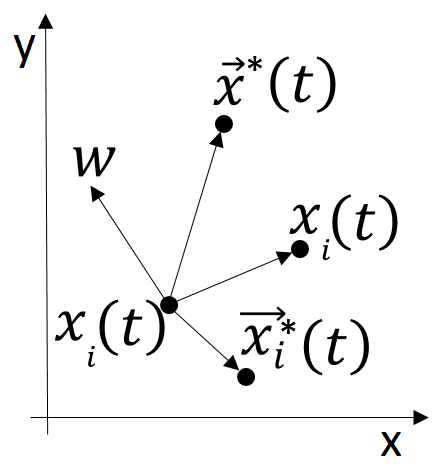
\includegraphics[scale=0.2]{./figs/grafico-pso.png}
%    %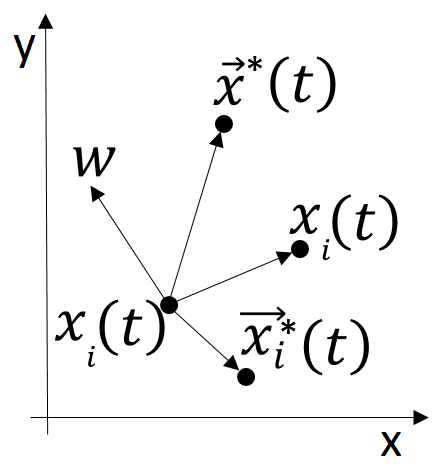
\includegraphics[width=\linewidth]{./figs/grafico-pso.png}
%   \caption{Movimento da partícula em um espaço de busca.}
%    \label{fig:grafico-pso}
%\end{figure}
O vetor velocidade $ \overrightarrow v _i $ é a soma vetorial das componentes cognitiva e social com a inércia da partícula. A inércia $ w $ atua como uma memória da direção da velocidade anterior da partícula e impede que haja alterações bruscas na direção da velocidade partícula~\cite{engelbrecht2007}. Assim, caso a partícula esteja se dirigindo a uma boa região, a descoberta de um novo líder social não alterará completamente essa direção. O papel da componente cognitiva é aproximar a partícula na direção da melhor posição encontrada por ela desde o início da busca. Dessa forma, a partícula deverá encontrar uma boa posição que provavelmente está próxima do seu líder cognitivo atual. Através da componente social, as partículas comunicam a informação sobre as melhores posições encontradas por elas desde o início do processo de busca, sendo considerada como a mais importante componente na equação da velocidade das partículas.

O pseudo-código do PSO é apresentado no Algoritmo~\ref{algoritmo-pso}. A cada passo, o algoritmo irá mudar a velocidade de cada partícula em direção às posições $ pbest $ e $ gbest $, onde a posição e a velocidade da partícula são atualizadas conforme as Equações~\ref{equa:pso1} e~\ref{equa:pso2}, respectivamente. Um termo aleatório $ r $ pondera o quanto a partícula se movimenta em direção a esses valores, onde diferentes números aleatórios são gerados em direção à aceleração para $ pbest $ e $ gbest $ locais~\cite{lazinica2009}. O algoritmo continuará a iterar até que um critério de parada seja alcançado. Geralmente, esse critério de parada é um número máximo de iterações especificado ou um valor aptidão pré-definido considerado bom o suficiente. A equação de velocidade contém vários parâmetros que afetam o desempenho do algoritmo e alguns afetam significativamente na convergência do algoritmo. A inércia $ w $, por exemplo, é fundamental para a convergência do algoritmo. Ela determina o quanto as velocidades anteriores afetarão a velocidade atual e definirá um equilíbrio entre o componente cognitivo local e o global social das partículas. Se o valor da inércia for alto, a velocidade aumentará, favorecendo a busca global. Mas, se o valor for baixo, as partículas sofrerão uma desaceleração, favorecendo a busca local. Dessa forma, um valor $ w $ que equilibra a pesquisa global e local implica menos iterações para que o algoritmo possa convergir.
\begin{algorithm}
	\caption{\textit{Particle Swarm Optimization}}
	\begin{algorithmic}[1]
		\State {$ d  \gets n$} \Comment {Inicializa a dimensão das partículas para $d$}
		\State {$ x[i]  \gets x _{aleatorio}$} \Comment {Inicializa a população de partículas com posições e velocidades aleatórias}
		\ {$ v[i]  \gets v _{aleatorio}$}
		\While {$ criterio parada = falso$} \Comment {Repete enquanto o critério de parada não tiver sido alcançado}
			\For{i}{1}{n} \Comment {Para cada partícula calcula o seu valor aptidão, compara o valor aptidão da partícula com o valor $pbest$ e com o valor de $gbest$}
			
				\If {$x_{atual} \leftrightarrow pbest$} \Comment {Se o valor atual da partícula é melhor do que $pbest$} 
					\State {$ x[i]  \gets x _{atual}$} 
					\ {$ pbest  \gets x _{atual}$}	 
				\EndIf
				\If {$x_{atual} \leftrightarrow gbest$} \Comment {Se o valor atual da partícula é melhor do que $gbest$}  
					\State {$ x[i]  \gets x _{atual}$}	
					\ {$ gbest  \gets x _{atual}$}
				\EndIf	
				
				\State {$ x[i]  \gets x _{calculada}$} \Comment {Atualiza a posição e velocidade da partícula  Equações~\ref{equa:pso1} e~\ref{equa:pso2}}
				
					 \ {$ v[i]  \gets v _{calcculada}$} 	
			\EndFor
		\EndWhile	
	\end{algorithmic}
	\label{algoritmo-pso}
\end{algorithm}
Apesar de $c_1$ e $c_2$ não influenciarem diretamente na convergência do PSO, o ajuste desses parâmetros agiliza e evita que o algoritmo seja pego em mínimos locais. O parâmetro $c_1$ é referido como parâmetro cognitivo e o valor $c_1r_1$, na Equação~\ref{equa:pso2}, define a relevância da melhor posição anterior. $c_2$ é referido como o parâmetro social e $c_2r_2$ e determina o comportamento da partícula em relação a outros vizinhos.

O número, a dimensão das partículas, o alcance e a velocidade máxima das partículas são parâmetros utilizados como entrada para o algoritmo, embora não componham a definição de velocidade. Quanto ao número de partículas, um valor alto costuma aumentar a probabilidade de encontrar o ótimo global. O valor deste número depende da complexidade do problema de otimização, mas um intervalo típico é entre 20 e 40 partículas~\cite {rodriguez2014}. Os valores para a dimensão das partículas e o alcance, no qual sua movimentação é permitida, são determinados unicamente pela natureza do problema que está sendo resolvido e de como ele é modelado para se adequar ao PSO. A velocidade máxima define a mudança máxima que uma partícula pode ter em uma iteração e normalmente seu valor é aproximadamente a metade do alcance de posição da partícula~\cite{rodriguez2014}.